\documentclass[border=12pt]{standalone}
\def\pgfsysdriver{pgfsys-dvisvgm.def}
\usepackage[dvisvgm]{xcolor}
\usepackage{xeCJK}
\setCJKmainfont{HaranoAjiGothic-Regular.otf}[BoldFont=HaranoAjiGothic-Bold.otf]
\setCJKsansfont{HaranoAjiGothic-Regular.otf}[BoldFont=HaranoAjiGothic-Bold.otf]
\usepackage{amsmath,amssymb,tikz,lmodern}
\usetikzlibrary{arrows.meta,positioning,calc,fit,backgrounds}
\renewcommand{\familydefault}{\sfdefault}
\definecolor{ink}{HTML}{25322F}
\definecolor{green}{HTML}{246657}
\definecolor{tint}{HTML}{EEF4F0}
\definecolor{soft}{HTML}{C6D2CC}
\definecolor{muted}{HTML}{52615B}
\newif\ifJapanese
\newcommand{\Tx}[2]{\ifJapanese #1\else #2\fi}
\newcommand{\Eff}{\overline{\operatorname{Eff}}}
\newcommand{\heading}[3]{{\color{green}\bfseries #1\quad\Tx{#2}{#3}}\\[5pt]}
% A white rectangle makes the complete citation label clickable, including spaces.
\newcommand{\refurl}[2]{\special{dvisvgm:raw <a xlink:href="#1" target="_blank" rel="noopener noreferrer">}{\setlength{\fboxsep}{0pt}\colorbox{white}{\color{green}\underline{\strut #2}}}\special{dvisvgm:raw </a>}}
\tikzset{
 card/.style={draw=soft,fill=white,rounded corners=2pt,align=left,text=ink,font=\fontsize{10.5}{14}\selectfont,inner xsep=12pt,inner ysep=10pt,text width=14.4cm},
 half/.style={card,text width=6.45cm,minimum height=2.05cm},
 result/.style={card,draw=green,fill=tint,line width=.9pt},
 reason/.style={align=left,text=muted,font=\fontsize{9}{12}\selectfont,inner sep=0pt,text width=12.7cm},
 branchreason/.style={reason,text width=5.95cm},
 edge/.style={-{Stealth[length=2.4mm]},draw=green,line width=1pt},
 wire/.style={draw=green,line width=1pt},
}
% Keep the arrow in a dedicated left gutter; explanations never cover it.
\newcommand{\flow}[3]{
 \coordinate (#2-from) at ($(#1.south)+(-6.9,0)$);
 \coordinate (#2-to) at ($(#2.north)+(-6.9,0)$);
 \draw[edge] (#2-from)--(#2-to);
 \node[reason,anchor=west] (#2-reason) at ($(#2-from)!.5!(#2-to)+(.55,0)$) {#3};
}

\newcommand{\Cite}[2]{\refurl{#1}{#2}}

\Japanesetrue
\begin{document}
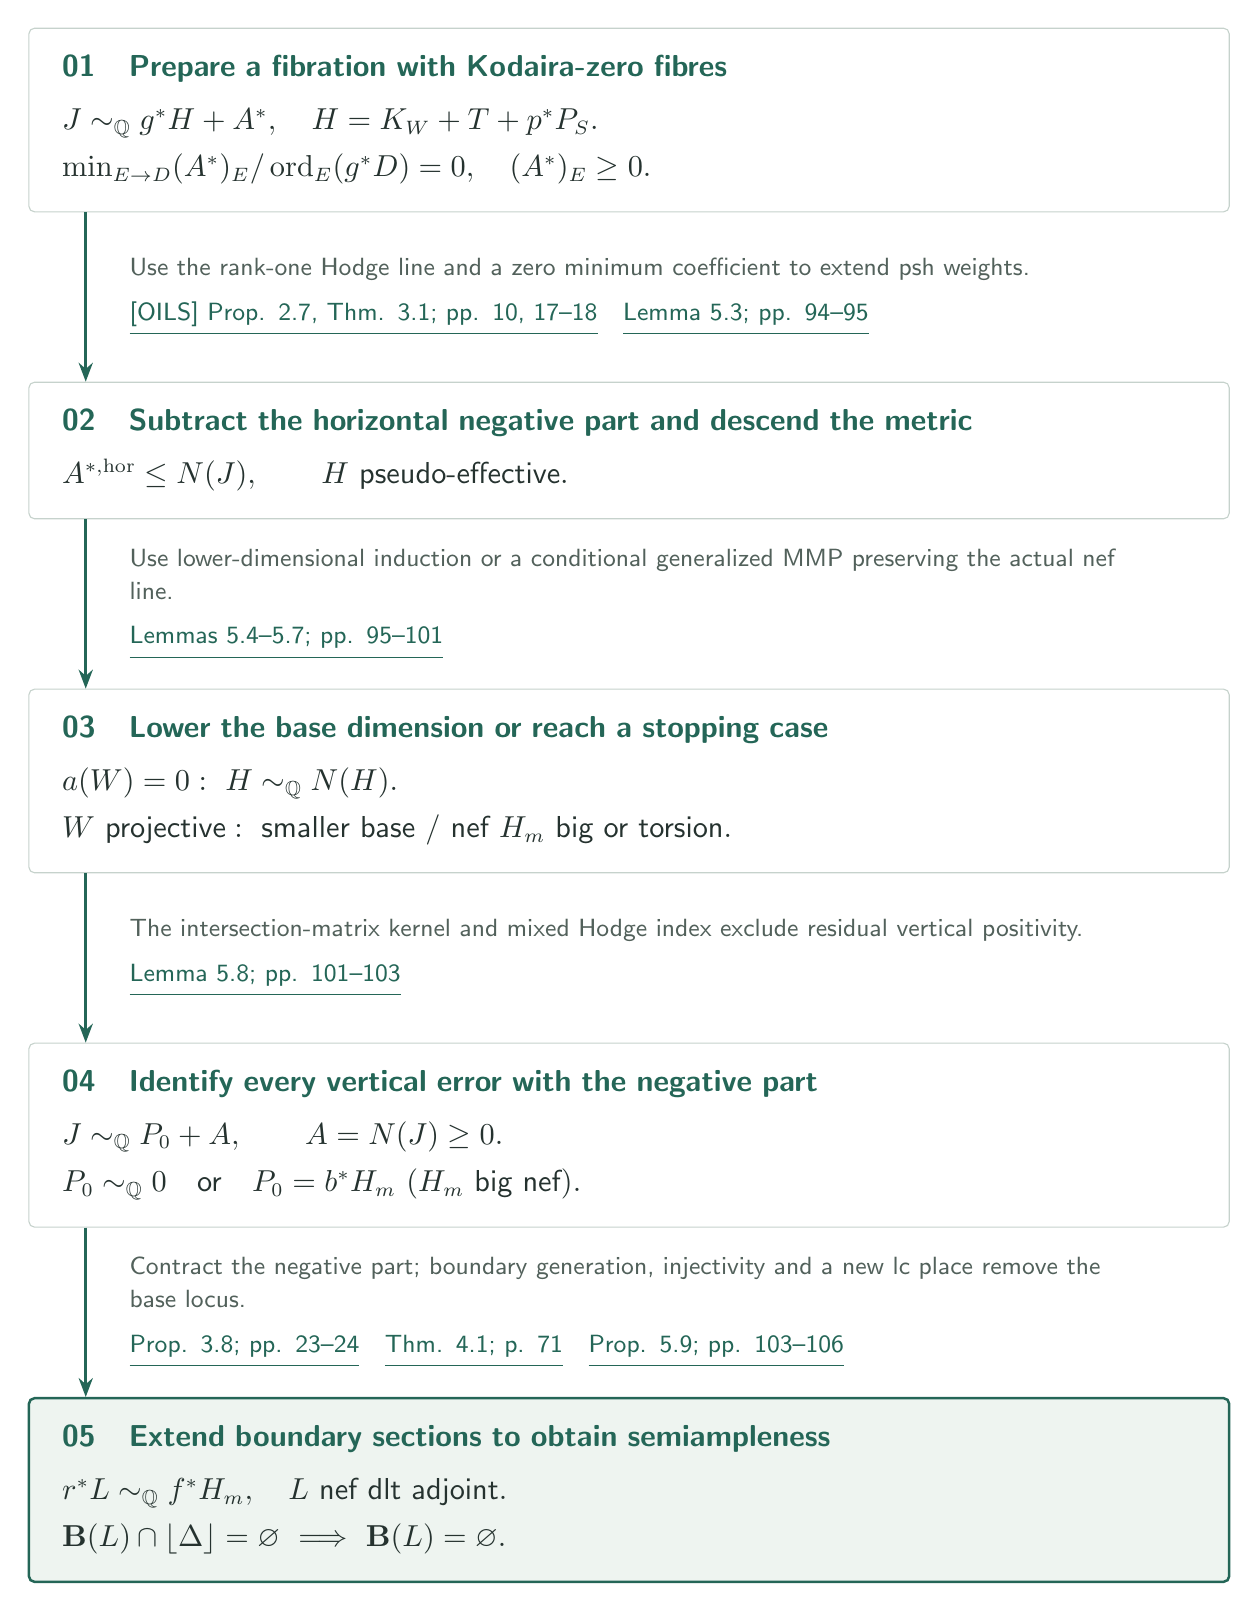
\begin{tikzpicture}
\node[card] (n0) {\heading{01}{飯高次元0のファイバーを持つ表示を準備}{Prepare a fibration with Kodaira-zero fibres}$J\sim_{\mathbb Q}g^*H+A^*,\quad H=K_W+T+p^*P_S.$\\[3pt] $\min_{E\to D}(A^*)_E/\operatorname{ord}_E(g^*D)=0,\quad (A^*)_E\ge0.$};
\node[card,below=2.15cm of n0] (n1) {\heading{02}{水平負部分を引いて底へmetricを降ろす}{Subtract the horizontal negative part and descend the metric}$A^{*,\mathrm{hor}}\le N(J),\qquad H\text{ pseudo-effective}.$};
\flow{n0}{n1}{\Tx{rank-one Hodge lineと係数の最小値0を使い、psh weightを延長。}{Use the rank-one Hodge line and a zero minimum coefficient to extend psh weights.}\\[4pt]\Cite{https://github.com/openai/math/blob/adc7f1241b42e322a6451854ab7e4b4c146bf78a/preprints/Orbifold-and-logarithmic-Iitaka-subadditivity-September-26-2026/paper.pdf}{[OILS] Prop. 2.7, Thm. 3.1; pp. 10, 17--18}\quad \Cite{https://github.com/openai/math/blob/adc7f1241b42e322a6451854ab7e4b4c146bf78a/preprints/Log-abundance-for-compact-Kahler-spaces-under-logarithmic-Iitaka-subadditivity-October-4-2026/main.pdf}{Lemma 5.3; pp. 94--95}}
\node[card,below=2.15cm of n1] (n2) {\heading{03}{底の次元を下げるか、停止する形へ進む}{Lower the base dimension or reach a stopping case}$a(W)=0:\ H\sim_{\mathbb Q}N(H).$\\[3pt] $W\text{ projective}:\ \Tx{\text{より低次元の底 / nefでbigまたはtorsionな }H_m}{\text{smaller base / nef }H_m\text{ big or torsion}}.$};
\flow{n1}{n2}{\Tx{下の次元の帰納、または実際のnef lineを保つ条件付き一般化MMP。}{Use lower-dimensional induction or a conditional generalized MMP preserving the actual nef line.}\\[4pt]\Cite{https://github.com/openai/math/blob/adc7f1241b42e322a6451854ab7e4b4c146bf78a/preprints/Log-abundance-for-compact-Kahler-spaces-under-logarithmic-Iitaka-subadditivity-October-4-2026/main.pdf}{Lemmas 5.4--5.7; pp. 95--101}}
\node[card,below=2.15cm of n2] (n3) {\heading{04}{全ての垂直誤差を負部分に同定}{Identify every vertical error with the negative part}$J\sim_{\mathbb Q}P_0+A,\qquad A=N(J)\ge0.$\\[3pt] $P_0\sim_{\mathbb Q}0\quad\text{or}\quad P_0=b^*H_m\ (H_m\text{ big nef}).$};
\flow{n2}{n3}{\Tx{交差行列の核と混合Hodge indexで、残る正の垂直部分を排除。}{The intersection-matrix kernel and mixed Hodge index exclude residual vertical positivity.}\\[4pt]\Cite{https://github.com/openai/math/blob/adc7f1241b42e322a6451854ab7e4b4c146bf78a/preprints/Log-abundance-for-compact-Kahler-spaces-under-logarithmic-Iitaka-subadditivity-October-4-2026/main.pdf}{Lemma 5.8; pp. 101--103}}
\node[result,below=2.15cm of n3] (n4) {\heading{05}{境界切断を延長してsemiampleにする}{Extend boundary sections to obtain semiampleness}$r^*L\sim_{\mathbb Q}f^*H_m,\quad L\text{ nef dlt adjoint}.$\\[3pt] $\mathbf B(L)\cap\lfloor\Delta\rfloor=\varnothing\ \Longrightarrow\ \mathbf B(L)=\varnothing.$};
\flow{n3}{n4}{\Tx{負部分を収縮し、境界生成・injectivity・新しいlc placeでbase locusを消す。}{Contract the negative part; boundary generation, injectivity and a new lc place remove the base locus.}\\[4pt]\Cite{https://github.com/openai/math/blob/adc7f1241b42e322a6451854ab7e4b4c146bf78a/preprints/Log-abundance-for-compact-Kahler-spaces-under-logarithmic-Iitaka-subadditivity-October-4-2026/main.pdf}{Prop. 3.8; pp. 23--24}\quad \Cite{https://github.com/openai/math/blob/adc7f1241b42e322a6451854ab7e4b4c146bf78a/preprints/Log-abundance-for-compact-Kahler-spaces-under-logarithmic-Iitaka-subadditivity-October-4-2026/main.pdf}{Thm. 4.1; p. 71}\quad \Cite{https://github.com/openai/math/blob/adc7f1241b42e322a6451854ab7e4b4c146bf78a/preprints/Log-abundance-for-compact-Kahler-spaces-under-logarithmic-Iitaka-subadditivity-October-4-2026/main.pdf}{Prop. 5.9; pp. 103--106}}
\end{tikzpicture}

\end{document}
